\documentclass[a4paper,14pt,russian]{article} %draft
\usepackage[T2A]{fontenc}% Поддержка русских букв

\usepackage{luacode}



% XeTeX packages
\usepackage[cm-default]{fontspec} % or install lmodern and remove cm-default opt
%\usepackage{xunicode} % some extra unicode support
\usepackage{xltxtra} % \XeLaTeX macro



\tolerance=1000
\emergencystretch=0.74cm
\usepackage{indentfirst} %делать отступ в начале параграфа

\usepackage[pdfborder = {0 0 0}]{hyperref} %гиперссылки в документе.

\usepackage[utf8]{inputenc} % кодировка текста
\usepackage[russian]{babel} % руссификация по Бабелю
\usepackage{graphics}

%\usepackage[clean,pdf]{svg}

\usepackage{amsmath, amsfonts} % для расширенных настроек ссылок на формулы
\usepackage{extsizes} % использование шрифтов большего кегля 

\usepackage{fancyvrb} % Добавляет продвинутые Verbatim и Verb

\usepackage{epsfig} % удобно вставлять рисунки в строку текста
\usepackage[usenames,dvipsnames]{pstricks}
\usepackage{pst-grad} % For gradients
\usepackage{pst-plot} % For axes

\usepackage{graphicx,xcolor}
\usepackage{minted}

%\usepackage[MakeStamp]{eskdi}
%\usepackage[MakeStamp, SubSectInToc]{eskdi}
%\usepackage[MakeStamp, SubSubSectInToc]{eskdi}
%\usepackage[MakeStamp, ParagraphInToc]{eskdi}
%\usepackage[twoside, MakeStamp, ParagraphInToc]{eskdi}
%\usepackage{eskdi}
%\usepackage[SubSectInToc]{eskdi}
%\usepackage[SubSubSectInToc]{eskdi}
%\usepackage[ParagraphInToc]{eskdi}
%\usepackage[SubParagraphInToc]{eskdi}
%\usepackage[twoside, ParagraphInToc]{eskdi}
\usepackage[MakeEmptyStamp, SubSubSectInToc]{eskdi}
%\usepackage[twoside, MakeEmptyStamp, SubSectInToc]{eskdi}
%\usepackage[twoside, MakeEmptyStamp, ParagraphInToc]{eskdi}
%\usepackage[twoside, MakeEmptyStamp]{eskdi}
%\usepackage[MakeEmptyStamp, ParagraphInToc]{eskdi}



\usepackage{array}
\usepackage{tabularx}
\usepackage{supertabular}
\usepackage{longtable} % для создания таблиц, переносящихся на другую страницу
%\usepackage{listingsutf8}%
\usepackage{listings} % для включения листинга кода в приложения. Русский язык глючит.


\lstloadlanguages{bash,[LaTeX]TeX,MetaPost,Clean,Matlab}


\usepackage{textcomp}	% Ввод различных знаков
\usepackage{keystroke} % для отображения символов клавиш
\usepackage{bytefield} %для создания таблиц с битовыми полями
\usepackage{filecontents} %для включения в документ содержимого файлов

\usepackage{tikz} % Пакет для рмсования диаграмм
\usepackage{tikz-timing}[2009/12/09]
\usetikzlibrary{arrows}
\usepackage{tikzit}
\input{sample.tikzstyles}

\usetikzlibrary{positioning,arrows,automata,plotmarks} %В данном случае нам потребуются positioning и arrows, которые нужны для расположения элементов друг относительно друга и рисования стрелок между ними соответственно.
\usetikzlibrary{shapes,snakes}
\usepackage{schemabloc}

\usepackage{makecell} % Для многострочных ячеек таблицы
\usepackage{colortbl} % Для раскрашивания ячеек в таблицах



\gostSetStampfont{Times New Roman}%

\setromanfont{Times New Roman}
\setsansfont{Arial}
\setmonofont{Consolas}
\setmainfont{Times New Roman}


%\verbatimfont{\fontspec[Scale=1.0]{Arial} \itshape}% % Для замены стиля начертания verbatim и verb
%\verbatimfont{\fontspec[Scale=1.0]{Times New Roman}}% % Для замены стиля начертания verbatim и verb
%\renewcommand{\SetStampfontIt}{\itshape}%
%\verbatimfont{\fontspec[Scale=1.0]{Consolas}}% % Для замены стиля начертания verbatim и verb
%\newfontfamily{\gostListingfont}[Scale=1.0]{Arial Narrow} % Шрифт для листингов
%\newfontfamily{\gostListingfont}[Scale=1.0]{Consolas} % Шрифт для листингов






% МАКРОСЫ, СПЕЦИФИЧЕСКИЕ ДЛЯ ДАННОГО ДОКУМЕНТА   Подключается в преамбуле


\newcolumntype{L}[1]{>{\raggedright\arraybackslash}p{#1}}% Выравнивание столбца по левому краю
\newcolumntype{C}[1]{>{\centering\arraybackslash}p{#1}}% Выравнивание столбца по левому центру
\newcolumntype{R}[1]{>{\raggedleft\arraybackslash}p{#1}}% Выравнивание столбца по правому краю



\newminted[LuaCode]{lua}{
               fontsize=\footnotesize,
               %linenos,
               breaklines,    % Перенос кода на другую строку
               numbersep=2mm,  %Отступ от номеров строк до кода
               xleftmargin=5mm,
               frame = lines, %Линия над кодом и линия под кодом
               baselinestretch=1.0 %Расстояние между строчками
               }


\definecolor{Gray}{gray}{0.94}%



 %Файл включает такие команды как надчёркивание, запрещение переноса ТУ и др.




\setpage % Разметка текста на странице

\begin{document}% Начало самого документа (содержательной части)

%======== Название документа, надписи на титульном листе, в основной надписи ========

\gosttitleobject{РАСШИРЕНИЕ ESKDI (V 4.2b)}
\gosttitleobjectI{Расширение eskdi (V 4.2b)}

\gosttitledocument{Инструкция по настройке и эксплуатации}
\gostreshenie{Решение от 11.02.2017}

\gostklgi{АБВГ.123456.789 И1} %То что будет в основной надписи
\gostferstklgi{АБВГ.123456.789} %Первичное применение

\gostrazrabotchik{Степаненко}
\gostrazrabotchikFIO{Степаненко\,Ю.\,А.}
  \gostDATErazrabotchik{11.02.2017}
\gostproveril{Проверивший}
  \gostDATEproveril{11.02.2017}
  
\gostnormokontroler{Суровая}
  \gostDATEnormokontroler{11.02.2017}

\gostutverdil{Утвердивший}
  \gostDATEutverdil{11.02.2017}
  
\gostliteraI{O}%Литера О
\gostliteraII{O$_1$} %Литера O1

\gostorganizatia{Организация}

\gostDATE{\today}


% Раскомментировать если необходима утверждающая надпись на титульном листе
\renewcommand\titleLEFT{%
  \spboxmm{0}{260}{70}{250}{lc}{\parbox{70mm}{\centering\normalsize{Утверждён \\} \large{АБВГ.123456.789 --ЛУ} }}
}%

% Раскомментировать если необходима утверждающая надпись на титульном листе
\renewcommand\titleRIGHT{%
  \spboxmm{110}{260}{185}{250}{lc}{\parbox{70mm}{\normalsize{ \begin{center}УТВЕРЖДАЮ\end{center} Генеральный директор\\ ЧОП ''В два глаза''\\ \_\_\_\_\_\_\_\_\_\_\_\_\_\_\_А.Р.Бородач\\''\_\_\_\_\_''\_\_\_\_\_\_\_\_\_\_2015~г.  }  }   }
}%

% Раскомментировать если совсем уж длинное название документа
%\renewcommand\SetTitleDocumentInSecondPage{%
%  \spboxmm{65}{0}{135}{25}{c}{\parbox{65mm}{\renewcommand\baselinestretch{0.6} \centering\footnotesize{Совсем уж длинное, такое длинное, аж до неприличия название для широко известного в узких кругах расширения eskdi (V 1.5b)} \footnotesize{\\ Инструкция по настройке и эксплуатации} }}
%}%


%Раскомментировать если хотите картинку на обложке
\renewcommand\titlePicture{\AddToShipoutPicture{\AtPageLowerLeft{\includegraphics[width=210mm, height=297mm, viewport=2.0mm 14.0mm 210.0mm 311.0mm]{\pathtosharedresource background21}}}}%



% Раскомментировать если необходима утверждающая надпись на титульном листе
%\renewcommand\titleTopLEFT{%
%  \spboxmm{0}{260}{70}{250}{lc}{\parbox{70mm}{\centering\normalsize{СОГЛАСОВАНО \\} Начальник $_{\frac{}{\ \ \ \text{номер} \ \ \ }}$ ВП МО \\ \ \\ \hrulefill \\ $^{^{\text{подпись, инициалы, фамилия}}}$ \\\hrulefill\\$^{^{\text{дата}}}$   }}
%}%


% Раскомментировать если необходима утверждающая надпись на титульном листе
%\renewcommand\titleCENTER{%
%  \spboxmm{0}{135}{170}{125}{lc}{\parbox{170mm}{
%  на 
%  \\Этап \hrulefill
%  \\Заказчик \hspace{1cm} ОАО «Нимфа»
%  \\Исполнитель \hspace{1cm} ОАО «Рога и копыта»
%  \\Заказ № \underline{\hspace{2cm}} Шифр (индекс) \hrulefill
%  \\Срок окончания работы \hrulefill
%  \\Дата выдачи задания \hrulefill
%  }}
%}%

% Раскомментировать если необходима утверждающая надпись на титульном листе
%\renewcommand\titleBotLEFT{%
%  \spboxmm{0}{70}{70}{70}{lc}{\parbox{70mm}{\centering\normalsize{Генеральный директор\\ОАО «Рога и копыта» \\} \underline{\hspace{4cm}} Х. З. Халявный\\ $^{^{\text{подпись, инициалы, фамилия}}}$ \\\hrulefill\\$^{^{\text{дата}}}$ }}
%}%


% Раскомментировать если необходима утверждающая надпись на титульном листе
%\renewcommand\titleBotRIGHT{%
 % \spboxmm{100}{70}{70}{30}{lc}{\parbox{70mm}{\centering\normalsize{Заместитель генерального\\директора ОАО «Нимфа»\\} \underline{\hspace{3cm}} Ц. Ж. Печальный \\ $^{^{\text{подпись, инициалы, фамилия}}}$ \\\hrulefill\\$^{^{\text{дата}}}$ \\ \centering\normalsize{Начальник отдела\\} \underline{\hspace{4cm}} Ш. Щ. Тихий \\ $^{^{\text{подпись, инициалы, фамилия}}}$ \\\hrulefill\\$^{^{\text{дата}}}$   }}
%}%




 %Здесь информация о названии файла, авторах и т.д.

\maketitle % Поместили Титульный лист


%\SetEmptyPage
\SetEvenPage


\makesecondpage


\tableofcontents % Содержание


\begin{luacode}
  function rnd(num, numDecimalPlaces)
    -- Округление числа до ближайшего и
    -- обрезка незначащих нулей
    local negate = false
    if (num < 0) then
      negate = true
      num = -num
    end

    local mult = 10^(numDecimalPlaces or 0)
    num_fl = math.floor(num * mult + 0.5) / mult
    local fmt = "%."..numDecimalPlaces.."f"

    if (negate == true) then
      num_fl = -num_fl
    end

    str = string.format(fmt, num_fl):gsub('\%.', ',')
    str = str:gsub('[0]+$', '')
    str = str:gsub(',$', '')
    return tex.sprint(str)
  end

  function rnd1(num)
    return rnd(num, 1)
  end

  function rnd2(num)
    return rnd(num, 2)
  end

  function rnd3(num)
    return rnd(num, 3)
  end

  -- Загрузка кода, исполнение, получение глобальной
  -- таблицы t с результатами вычислений
  local file = io.open("calc_pollution.lua", "r")
  local code = file:read("*all")
  file:close()
  local res, calc = pcall(load('return '..code))
  t = calc()
\end{luacode}




\section*{Введение}

Ежегодно в России происходит рост численности населения по данным Росстата и по оценке уже к 2036~году численность составит 153,2~млн человек. Каждый человек с самого рождения стремится к удовлетворению своих амбиций, к хорошей стабильной жизни. И так уж сложилось, что  признаком успешности человека в жизни является наличие большого количества денег, сбережений, недвижимости, и, в частности, автомобилей. Для кого-то это просто средство передвижения, для кого-то показатель статуса.

Актуальность темы исследования. Одной из острых экологических проблем настоящего времени является загрязнение атмосферного воздуха. В больших городах к числу основных источников загрязнения атмосферного воздуха относится автотранспорт. Отходящие газы двигателей содержат сложную смесь из более двухсот компонентов, среди которых немало канцерогенов. Вредные вещества поступают в воздух практически в зоне дыхания человека. Поэтому автомобильный транспорт следует отнести к наиболее опасным источникам загрязнения. В настоящее время мировой автомобильный парк превысил 600~млн. единиц, из которых 83-85~\% приходится на легковые автомобили. По прогнозам, к 2030~году он достигнет 1,5~млрд. единиц.

Мировой ежегодный выброс вредных веществ от автомобилей составляет 50~млн.т. углеводородов, 200~млн.т, оксида углерода и 20~млн.т. оксидов азота. Во многих городах мира концентрации вредных веществ в воздухе, создаваемые выбросами автотранспорта, превышают стандарты качества атмосферного воздуха.

Во многих городах России выбросы автотранспорта преобладают над выбросами от стационарных источников, и уровень загрязнения воздуха превышает нормативы предельно допустимых концентраций. В связи с этим проблема снижения негативного воздействия автотранспорта на здоровье людей, воздушный и водный бассейны, растительный и животный мир, почвы весьма актуальна.

Защита атмосферы от вредных воздействий, возникающих в результате эксплуатации автомобильного транспорта, является крайне актуальной, поскольку от качества атмосферного воздуха в наибольшей степени зависит не только здоровье человека, но и в целом качество жизни на планете. Это составляет практическую значимость работы.

Цель работы: оценка влияния автотранспорта на состояние окружающей среды путем измерения и сравнения уровня загрязнения СО на разных остановочных пунктах г.~Воронежа.

Задачи исследования:
\begin{itemize}
\item оценка влияния автотранспорта на окружающую среду;
\item определение величины выбросов загрязняющих веществ от автотранспортных средств;
\item исследование загруженности автотранспортом с учетом видов автомобилей на остановочных пунктах: ''Спартак'', ''Карла Маркса'' и ''ТЮЗ'' г. Воронежа.
\end{itemize}

Объектом исследования является приземный слой атмосферы на остановочных пунктах: ''ул. Карла Маркса'', ''Кинотеатр ''Спартак'' и ''ТЮЗ'' г. Воронежа. Целью исследования – влияние выбросов от автотранспорта на состояние приземного слоя атмосферы на этих остановочных пунктах.

Всех тех, кто покупает автомобиль сейчас, однозначно должна беспокоить проблема загрязнения окружающей среды выхлопными газами автомобилей на двигателях внутреннего сгорания. Безусловно, сейчас появляется все больше средств передвижения на электрической тяге, но они гораздо дороже, и имеют свои отрицательные стороны. Человечеству нужна дешевая альтернатива бензиновым автомобилям в ближайшем будущем.

Сроки проведения работы ноябрь 2022~года.







\section{Теоретическая часть}

\subsection{Автотранспорт и его влияние на экологию города}

Автомобильный парк, являющийся одним из основных источников загрязнения окружающей среды, сосредоточен, в основном, в городах. Если в среднем в мире на 1~км$^2$ территории приходится пять автомобилей, то плотность их в крупнейших городах развитых стран в 200-300~раз выше. В настоящее время в мире насчитывается 940~млн. легковых, 80~млн. грузовых автомобилей и примерно 1,5~млн. городских автобусов.

Автомобили сжигают огромное количество ценных нефтепродуктов, нанося одновременно ощутимый вред окружающей среде, главным образом атмосфере. Поскольку основная масса автомобилей сконцентрирована в крупных и крупнейших городах, воздух этих городов не только обедняется кислородом, но и загрязняется вредными компонентами отработавших газов. Противоречия, из которых ''соткан'' автомобиль, пожалуй, ни в чём не выявляются так резко, как в деле защиты природы. С одной стороны, он облегчил человеку жизнь, с другой – отравляет её в самом прямом смысле слова. Специалисты установили, что один легковой автомобиль ежегодно поглощает из атмосферы в среднем более 4~тонн кислорода, выбрасывая с отработавшими газами примерно 800~кг окиси углерода, около 40~кг окислов азота и почти 200~кг различных углеводородов. Если помножить эти цифры на 600~млн. единиц мирового парка автомобилей, можно представить себе степень угрозы, таящейся в чрезмерной автомобилизации.
Для снижения вредного влияния автомобильного транспорта требуется вынос из городской черты грузовых транзитных потоков. Требование это зафиксировано в действующих строительных нормах и правилах, но практически соблюдается редко.

Для снижения вредного влияния автомобильного транспорта требуется вынос из городской черты грузовых транзитных потоков. Требование это зафиксировано в действующих строительных нормах и правилах, но практически соблюдается редко.

''Город без автомобиля'' мыслится как сочетание широких транспортных магистралей, где предоставляется простор для автомобильного движения, с микрорайонами, куда въезд транспорта запрещён или предельно ограничен и где люди ходят только пешком.

Эффективным мероприятием по снижению вредного влияния автомобильного транспорта на горожан является организация пешеходных зон с полным запретом въезда транспортных средств на жилые улицы. Развитие общественного транспорта в городах обуславливает необходимость поиска путей оптимального использования городских территорий, так как для перевозки одного пассажира в трамвае требуется 0,9~м$^2$, автобусе – 1,1~м$^2$, легковом автомобиле – свыше 20~м$^2$ городской территории \cite{golubev}.

''Автомобиль не роскошь, а средство передвижения'' – эти слова из известного произведения Ильфа и Петрова, звучавшие иронически, обрели в наше время реальный смысл. Более 10~млн. людей имеют автомобиль в личном пользовании. Взлёт использования личного автотранспорта произошёл в последние 15~лет.





\subsection{Классификация автомобилей}

Автомобильная промышленность в зависимости от назначения и приспособленности к дорожным условиям выпускает автомобили различных типов. По назначению автомобили делятся на пассажирские, грузовые и специальные. К пассажирским автомобилям, предназначенным для перевозки людей, относятся легковые автомобили и автобусы. Грузовые автомобили служат для перевозки различных грузов. 

Пассажирские автомобили, вмещающие не более 8~человек, называют легковыми, а вмещающие более 8~человек – автобусами.

Автобусы, предназначенные для внутри городского и пригородного общественного транспорта, называют городскими, а предназначенные для междугородних перевозок - междугородными. Число мест в автобусах в зависимости от назначения составляет 10–80.
По длине автобусы разделены на следующие классы:
\begin{itemize}
\item особо малый до 5~м;
\item малый 6–7,5~м;
\item средний 8–9,5~м;
\item большой 10,5–12~м.
\end{itemize}

Грузовые автомобили делят по грузоподъемности, т. е. по массе груза (т), который можно перевести в кузове. По грузоподъемности они делятся на классы:
\begin{itemize}
\item особо малый 0,3–1~т;
\item малый 1–3~т;
\item средний 3–5~т;
\item большой 5–8~т;
\item особо большой 8~т и более.
\end{itemize}

Автомобили специального назначения выполняют не транспортные работы. К ним относятся коммунальные автомобили для очистки и поливки улиц, пожарные, автокраны и т.д.

По приспособленности к дорожным условиям различают автомобили нормальной и повышенной проходимости. Первые имеют один, а вторые два или три ведущих моста, что позволяет им преодолевать бездорожье или плохие участки дороги.

По типу двигателя автомобили делят на имеющие карбюраторные двигатели, газовые, дизели, электродвигатели.








\subsection{Основные виды топлива, используемые в автотранспорте}

\subsubsection{Автомобильные бензины}

На автозаправках продают бензин марок \mbox{АИ-80} (он же \mbox{А-76} или \mbox{Н-80}), \mbox{АИ-92}, \mbox{АИ-95}, \mbox{АИ-98}.
Буква А означает, что бензин автомобильный, цифра - наименьшее октановое число, определенное по моторному методу; наличие буквы И указывает на то, что октановое число определено по исследовательскому методу. Автомобильные бензины, за исключением бензина \mbox{АИ-98}, разделены на летние и зимние. Зимние бензины содержат увеличенное количество легкоиспаряющихся фракций, что улучшает условие пуска двигателя.

В автомобильные бензины \mbox{А-76}, \mbox{АИ-92}, \mbox{АИ-98} добавляют антидетонатор~- тетраэтилсвинец (ТЭС) для повышения их антидетонационной стойкости. Вредные эффекты, вызываемые тетраэтилсвинцом, стали известны общественности начиная с конца 1940-х — начала 1950-х годов.

Тетраэтилсвинец — летучая жидкость при вдыхании воздуха проникает в организм через органы дыхания. Тетраэтилсвинец также может проникать в организм через неповрежденную кожу. Это вещество является сильным ядом, который избирательно поражает нервную систему, вызывая острые, подострые и хронические отравления. Хронические отравления обусловлены кумулятивным физиологическим эффектом, свойственным этому токсическому веществу. Поражается прежде всего кора головного мозга.


\begin{figure}[H]%
  \centering
  \includegraphics[width=0.4\textwidth]{src/tetraetilPb.png}
  \caption{Молекула тетраэтилсвинца} \label{p:k_marks}
\end{figure}% scale = 0.3, width=\textwidth


Для отличия обыкновенного бензина от этилированных, последние окрашивают в зеленый (\mbox{А-76}), синий (\mbox{АИ-92}) и желтый (\mbox{АИ-98}) цвета.




\subsubsection{Дизельное топливо}

Топливо, применяемое для автомобильных дизельных двигателей, представляет собой тяжелые нефтяные фракции. Оно должно обеспечивать мягкую и плавную работу двигателей, отвечать условиям надежной подачи его в цилиндры топливоподающей аппаратурой, не оставлять значительного нагара, быть свободным от механических примесей и воды, содержать наименьшее количество органических кислот и серы. Дизельное топливо должно иметь определенную вязкость и возможно более низкую температуру застывания и воспламенения.

В настоящее время по \mbox{ГОСТ 305-82}, \mbox{ГОСТ 1667-68} выпускаются сорта дизельного топлива: Л - летнее, З - зимнее, А - арктическое. Каждое из названных топлив делится на две подгруппы: первая с содержанием серы не более 0,2~\% и вторая содержание не превышает 0,5~\%.

Летнее дизельное топливо ДЛ можно применять только при температуре окружающего воздуха выше 0~°С. Когда температура опускается до минус 20~°С, следует применять зимнее топливо З, а при морозах, достигающих -30~°С топливо ДЗ, при более низких температурах применяют арктическое топливо. Однако применять арктическое топливо при температуре выше минус -30~°С нельзя.



\subsubsection{Топливо для газобаллонных автомобилей}

Горючие газы, используемые в газобаллонных автомобилях, могут быть естественными и искусственными. Естественные газы добывают из подземных газовых или нефтяных скважин. Искусственные газы являются побочными продуктами, получаемыми на химических или металлургических заводах. 

Установлены следующие марки газов:
\begin{itemize}
\item СПБТЗ - смесь пропана и бутана техническое зимнее;
\item СПБТЛ - смесь пропана и бутана техническое летнее;
\item БТ - бутан технический.
\end{itemize}

Сжиженный пропан - бутановый газ согласно стандарту должен содержать пропана зимой не менее 90~\%, а летом не менее 70~\%. Газ не должен содержать механических примесей, воды, водорасстворимых кислот, щелочей и других загрязняющих веществ.

Сжатыми называют газы, которые при обычной температуре окружающей среды и высоком давлении до 20~тыс.~кН/м$^2$ сохраняют газообразное состояние.
Сжиженными газами называют такие, которые переходят из газообразного состояния в жидкое при нормальной температуре и небольшом давлении до 1600~кН/м$^2$.
Для газобаллонных автомобилей использование сжиженных газов предпочтительнее, чем сжатых 
\cite{mihailovsky}.










\newpage
\subsection{Причины дымления автомобилей}

Причины дымления автомобилей различны: неисправность двигателя, неотлаженность системы питания или зажигания. Если все автомобильные двигатели будут правильно отрегулированы, то выброс вредных веществ в атмосферу уменьшится в 3-5~раз. Экономия денег на техобслуживании приводят к тому, что автомобили неделями, а то и месяцами развозят по улицам ядовитый газ. Плохо накачанные шины не только быстрее изнашиваются, но и увеличивают сопротивление движению, а значит, больше сжигается горючего. Сильно сказывается на окружающей среде сотяние автомобилей в ''пробках'' со включенными двигателями.

Неумелое поведения водителя за рулём (неправильный выбор скоростей движения, резкие разгоны и торможения, превышение установленной скорости), а так же самостоятельная регулировка (увеличение частоты вращения на холостом ходу) и нарушение инструкций по эксплуатации автомобиля, нередко приводит к увеличению загрязнения окружающей среды. Поэтому разъяснительная работа среды водителей автомобилей в этом направлении очень важна.









\subsection{Краткая характеристика монооксида углерода СО (угарного газа) и его влияние на природную среду и человека}

Образуется в результате неполного сгорания углерода в моторном топливе. Ядовитый газ без цвета и запаха. 

\begin{figure}[H]%
  \centering
  \begin{minipage}[h]{0.4\linewidth}
    \center{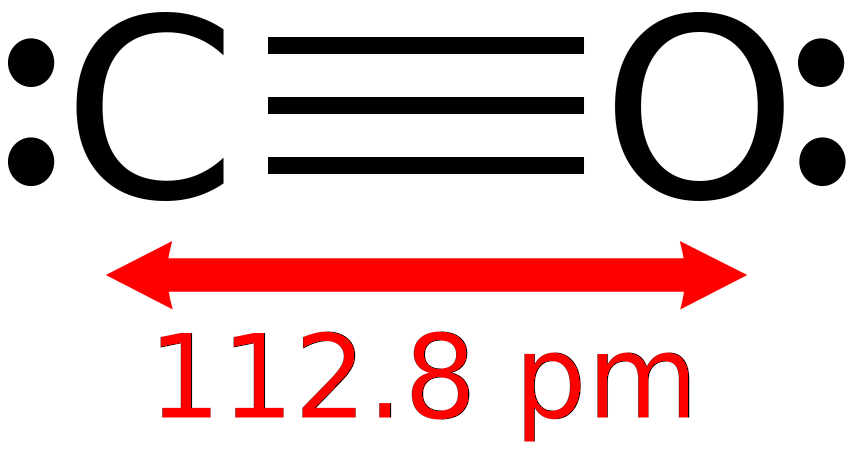
\includegraphics[width=0.8\textwidth]{src/Carbon_monoxide_2D.png}}
  \end{minipage}
  \hfill
  \begin{minipage}[h]{0.4\linewidth}
    \center{\includegraphics[width=0.8\textwidth]{src/Carbon-monoxide-3D-vdW.png}}
  \end{minipage}
  \caption{Молекула монооксида углерода СО} \label{p:Carbon_monoxide}
\end{figure}% scale = 0.3, width=\textwidth

При вдыхании связывается с гемоглобином крови, вытесняя из нее кислород, в результате чего наступает кислородное голодание, сказывающееся прежде всего на центральной нервной системе. Среднесуточная предельно допустимая концентрация (ПДК) по монооксиду углерода составляет \directlua{rnd2(t.PDK)}~мг/м$^3$.

Высокая концентрация монооксида углерода даже при кратковременном воздействии может привести к смерти: небольшие дозы вызывают головокружение, головную боль, чувство усталости и замедление реакции у водителя. Повышение концентрации монооксида углерода часто возникает в туннелях (до 70~ПДК), в потоке транспортных средств при интенсивном движении (до 60~ПДК), в гаражах. Известны случаи трагической гибели людей, запускающих двигатели автомобилей при закрытых воротах гаража. В одноместном гараже смертельная концентрация СО возникает уже через 2-3~мин. после включения стартера. В холодное время года, остановившись для ночлега, водители иногда включают двигатель для обогрева салона. Из-за проникновения монооксида углерода в кабину такой ночлег может оказаться последним.

Воздействие атмосферных загрязнений на здоровье можно подразделить на два вида в зависимости от времени проявления эффекта: острое, сказывающееся в период или непосредственно вслед за повышением концентрации токсичного вещества, и хроническое воздействие, результат которого проявляется не сразу, а через некоторое время, иногда через годы. Как в первом, так и во втором случаях атмосферные загрязнения могут быть непосредственной причиной развития заболевания или оказывать не специфическое отягощающее воздействие.

Проникновение угарного газа повышенной концентрации через органы дыхания в наши дни привело к существенному изменению состояния организма. Развилась патологическая повышенная чувствительность организма. Ощутимыми темпами происходит накопление наследственных пороков. Широкое распространение получили хронический бронхит, а также прежде формы легочной патологии, такие как аллергические воспаления альвеол. Увеличилось число больных бронхиальной астмой, относящейся к наиболее тяжелым проявлениям аллергии. Особую тревогу вызывает увеличение количества больных раком легкого, который по своей распространительности у мужчин вышел на первое место среди онкологических заболеваний. Потому как остро стоит проблема защиты воздушной среды от всех видов загрязнений.







\section{Практическая часть}

\subsection{Методы исследования}

Метод расчета уровня загрязнения СО я позаимствовала у работников ВГУ: Негробов~О.П., Логвиновский~В.Д. и Пантелеева~Н.Ю. В их практикуме мною была найдена специальная формула для расчета того самого загрязнения.

Для оценки загрязнения приземного слоя атмосферного воздуха используется формула (\ref{eq:main}) из \cite{begma}:

\begin{equation}
K_{CO} = (0,5 + 0,01N * K_{\text{Т}}) * K_{\text{А}} * K_{\text{У}} * K_{\text{С}} * K_{\text{В}} * K_{\text{П}},
\label{eq:main}
\end{equation}

\par где $K_{CO}$ – концентрация окиси углерода, мг/м$^3$,
\par 0,5 – фоновое (не транспортное) загрязнение приземного слоя атмосферного воздуха в пределах городской черты Воронежа, мг/м$^3$,
\par N – суммарная интенсивность движения автомобилей на улицах г.~Воронежа (автомобилей/час),
\par $K_{\text{Т}}$ – коэффициент токсичности определенного типа автомобилей по выбросам в атмосферу СО,
\par $K_{\text{А}}$ – коэффициент, учитывающий аэрацию на данном участке дороги (таблица~\ref{t:Ka}),
\par $K_{\text{У}}$ – коэффициент, учитывающий величину уклона дорожного полотна (таблица~\ref{t:Ku}),
\par $K_{\text{С}}$ – коэффициент, учитывающий скорость ветра (таблица~\ref{t:Kc}),
\par $K_{\text{В}}$ – коэффициент, учитывающий влажность воздуха (таблица~\ref{t:Kv}),
\par $K_{\text{П}}$ – коэффициент, учитывающий зависимость концентрации окиси углерода от типа пересечения дорог (таблица~\ref{t:Kp}).


Значение коэффициента токсичности по выбросам в атмосферу СО ($K_{\text{Т}}$) определяется по формуле:
\begin{equation}
K_{\text{Т}} = \sum_{i=1}^{N}P_{i}K_{\text{Т}i},
\label{eq:Kt}
\end{equation}

\par где $P_{i}$ – состав движения (в долях от общего количества транспортного потока),
\par $K_{\text{Т}i}$ – токсичности (по выбросу СО) для каждого вида транспорта.



Для исследования мной были выбраны три остановочных пункта:
\begin{itemize}
\item остановка ''ул. Карла Маркса'';
\item остановка ''Кинотеатр ''Спартак'';
\item остановка ''ТЮЗ''.
\end{itemize}

Ниже на рисунках показаны фрагменты карт с этими остановками.

\begin{figure}[H]%
  \centering
  \includegraphics[width=0.8\textwidth]{src/st_k_marks.jpg}
  \caption{Остановка ''ул. Карла Маркса''} \label{p:k_marks}
\end{figure}% scale = 0.3, width=\textwidth

\begin{figure}[H]%
  \centering
  \includegraphics[width=0.8\textwidth]{src/st_spartak.jpg}
  \caption{Остановка ''Кинотеатр ''Спартак''} \label{p:spartak}
\end{figure}% scale = 0.3, width=\textwidth

\begin{figure}[H]%
  \centering
  \includegraphics[width=0.8\textwidth]{src/st_tuz.jpg}
  \caption{Остановка ''ТЮЗ''} \label{p:tuz}
\end{figure}% scale = 0.3, width=\textwidth

Мой выбор можно логически обосновать. Все они находятся в шаговой доступности от моего
дома, поэтому измерить уровень загрязнения именно там – жизненная необходимость.

Для всех улиц можно сказать: ''магистральная улица с многоэтажной застройкой с обеих сторон'' (таблица~\ref{t:Ka}).

Для всех улиц можно сказать, что ''продольный уклон 0~\%'' (таблица~\ref{t:Ku}).

Для всех улиц можно сказать, что движение ''регулируемое автоматическими светофорами'' (таблица~\ref{t:Kp}).





Я измерила количество машин, которые проедут мимо каждого пункта за один час.


\subsubsection{Остановка ''ул. Карла Маркса''}



23 ноября 2022~года с 18:00 до 19:00 я проводила подсчеты на остановке ''ул. Карла Маркса'' (рисунок~\ref{p:k_marks}). Результаты приведены в таблице~\ref{t:k_marks}. В этот день был порывистый ветер со скоростью 4~м/сек (таблица~\ref{t:Kc}) и дождь (влажность воздуха 100~\%, таблица~\ref{t:Kv}).

\small
\begin{longtable}{|L{70mm}|C{40mm}|C{30mm}|C{15mm}|}
  \caption{Определение коэффициента токсичности по выбросам в атмосферу СО ($K_{\text{Т}}$) на остановке ''ул. Карла Маркса''} \label{t:k_marks} \\
  \hline
  \rowcolor{Gray}
  \multicolumn{1}{|L{70mm}|}{\centering Тип автотранспортного средства} &
  \multicolumn{1}{C{40mm}|}{\centering Количество автомобилей} &
  \multicolumn{1}{C{30mm}|}{\centering Доля от общего количества транспортного потока ($P_{i}$)} &
  \multicolumn{1}{C{15mm}|}{\centering $K_{\text{Т}i}$} \\\hline
  \endfirsthead
  \caption*{Продолжение таблицы \ref{t:k_marks}} \\
  \hline
  \rowcolor{Gray}
  \multicolumn{1}{|L{70mm}|}{\centering Тип автотранспортного средства} &
  \multicolumn{1}{C{40mm}|}{\centering Количество автомобилей} &
  \multicolumn{1}{C{30mm}|}{\centering Доля от общего количества транспортного потока ($P_{i}$)} &
  \multicolumn{1}{C{15mm}|}{\centering $K_{\text{Т}i}$} \\\hline
  \endhead
   Лёгкий грузовой (в том числе маршрутные такси ''Газель'')             & \directlua{rnd2(t.k_marks.lg.Num)}     & \directlua{rnd3(t.k_marks.lg.Pi)}     & \directlua{rnd2(t.k_marks.lg.Kti)}     \\ \hline
   Средний грузовой (в том числе маршрутные	такси-автобусы ''ПАЗ'')      & \directlua{rnd2(t.k_marks.sg.Num)}     & \directlua{rnd3(t.k_marks.sg.Pi)}     & \directlua{rnd2(t.k_marks.sg.Kti)}     \\ \hline
   Тяжёлый грузовой (дизельные, в том числе маршрутные автобусы)       & \directlua{rnd2(t.k_marks.tg_diz.Num)} & \directlua{rnd3(t.k_marks.tg_diz.Pi)} & \directlua{rnd2(t.k_marks.tg_diz.Kti)} \\ \hline
   Тяжёлый грузовой (с двигателями внутреннего сгорания)               & \directlua{rnd2(t.k_marks.tg_dvs.Num)} & \directlua{rnd3(t.k_marks.tg_dvs.Pi)} & \directlua{rnd2(t.k_marks.tg_dvs.Kti)} \\ \hline
   Легковой                                                            & \directlua{rnd2(t.k_marks.l.Num)}      & \directlua{rnd3(t.k_marks.l.Pi)}      & \directlua{rnd2(t.k_marks.l.Kti)}      \\ \hline
   Всего автомобилей за 1~час                                          & \directlua{rnd2(t.k_marks.summ.Num)}   &                                       & \directlua{rnd2(t.k_marks.summ.Kt)}    \\ \hline
\end{longtable} \normalsize




\subsubsection{Остановка ''Кинотеатр ''Спартак''}

24 ноября 2022~года с 18:00 до 19:00 я проводила подсчеты на остановке ''Кинотеатр ''Спартак'' (рисунок~\ref{p:spartak}). Результаты приведены в таблице~\ref{t:spartak}. В этот день был туман, что означает ветер 0~м/сек (таблица~\ref{t:Kc}) и влажность воздуха 100~\% (таблица~\ref{t:Kv}).

\small
\begin{longtable}{|L{70mm}|C{40mm}|C{30mm}|C{15mm}|}
  \caption{Определение коэффициента токсичности по выбросам в атмосферу СО ($K_{\text{Т}}$) на остановке ''Кинотеатр ''Спартак''} \label{t:spartak} \\
  \hline
  \rowcolor{Gray}
  \multicolumn{1}{|L{70mm}|}{\centering Тип автотранспортного средства} &
  \multicolumn{1}{C{40mm}|}{\centering Количество автомобилей} &
  \multicolumn{1}{C{30mm}|}{\centering Доля от общего количества транспортного потока ($P_{i}$)} &
  \multicolumn{1}{C{15mm}|}{\centering $K_{\text{Т}i}$} \\\hline
  \endfirsthead
  \caption*{Продолжение таблицы \ref{t:spartak}} \\
  \hline
  \rowcolor{Gray}
  \multicolumn{1}{|L{70mm}|}{\centering Тип автотранспортного средства} &
  \multicolumn{1}{C{40mm}|}{\centering Количество автомобилей} &
  \multicolumn{1}{C{30mm}|}{\centering Доля от общего количества транспортного потока ($P_{i}$)} &
  \multicolumn{1}{C{15mm}|}{\centering $K_{\text{Т}i}$} \\\hline
  \endhead
   Лёгкий грузовой (в том числе маршрутные такси ''Газель'')             & \directlua{rnd2(t.k_spartak.lg.Num)}     & \directlua{rnd3(t.k_spartak.lg.Pi)}     & \directlua{rnd2(t.k_spartak.lg.Kti)}     \\ \hline
   Средний грузовой (в том числе маршрутные	такси-автобусы ''ПАЗ'')      & \directlua{rnd2(t.k_spartak.sg.Num)}     & \directlua{rnd3(t.k_spartak.sg.Pi)}     & \directlua{rnd2(t.k_spartak.sg.Kti)}     \\ \hline
   Тяжёлый грузовой (дизельные, в том числе маршрутные автобусы)       & \directlua{rnd2(t.k_spartak.tg_diz.Num)} & \directlua{rnd3(t.k_spartak.tg_diz.Pi)} & \directlua{rnd2(t.k_spartak.tg_diz.Kti)} \\ \hline
   Тяжёлый грузовой (с двигателями внутреннего сгорания)               & \directlua{rnd2(t.k_spartak.tg_dvs.Num)} & \directlua{rnd3(t.k_spartak.tg_dvs.Pi)} & \directlua{rnd2(t.k_spartak.tg_dvs.Kti)} \\ \hline
   Легковой                                                            & \directlua{rnd2(t.k_spartak.l.Num)}      & \directlua{rnd3(t.k_spartak.l.Pi)}      & \directlua{rnd2(t.k_spartak.l.Kti)}      \\ \hline
   Всего автомобилей за 1~час                                          & \directlua{rnd2(t.k_spartak.summ.Num)}   &                                         & \directlua{rnd2(t.k_spartak.summ.Kt)}    \\ \hline
\end{longtable} \normalsize




\subsubsection{Остановка ''ТЮЗ''}

25 ноября 2022~года с 18:00 до 19:00 я проводила подсчеты на остановке ''ТЮЗ'' (рисунок~\ref{p:tuz}). Результаты приведены в таблице~\ref{t:tuz}. В этот день был слабый ветер ( 0~м/сек, таблица~\ref{t:Kc}) и подмораживало (влажность воздуха 40~\%, таблица~\ref{t:Kv}).

\small
\begin{longtable}{|L{70mm}|C{40mm}|C{30mm}|C{15mm}|}
  \caption{Определение коэффициента токсичности по выбросам в атмосферу СО ($K_{\text{Т}}$) на остановке ''ТЮЗ''} \label{t:tuz} \\
  \hline
  \rowcolor{Gray}
  \multicolumn{1}{|L{70mm}|}{\centering Тип автотранспортного средства} &
  \multicolumn{1}{C{40mm}|}{\centering Количество автомобилей} &
  \multicolumn{1}{C{30mm}|}{\centering Доля от общего количества транспортного потока ($P_{i}$)} &
  \multicolumn{1}{C{15mm}|}{\centering $K_{\text{Т}i}$} \\\hline
  \endfirsthead
  \caption*{Продолжение таблицы \ref{t:tuz}} \\
  \hline
  \rowcolor{Gray}
  \multicolumn{1}{|L{70mm}|}{\centering Тип автотранспортного средства} &
  \multicolumn{1}{C{40mm}|}{\centering Количество автомобилей} &
  \multicolumn{1}{C{30mm}|}{\centering Доля от общего количества транспортного потока ($P_{i}$)} &
  \multicolumn{1}{C{15mm}|}{\centering $K_{\text{Т}i}$} \\\hline
  \endhead
   Лёгкий грузовой (в том числе маршрутные такси ''Газель'')             & \directlua{rnd2(t.k_tuz.lg.Num)}     & \directlua{rnd3(t.k_tuz.lg.Pi)}     & \directlua{rnd2(t.k_tuz.lg.Kti)}     \\ \hline
   Средний грузовой (в том числе маршрутные	такси-автобусы ''ПАЗ'')      & \directlua{rnd2(t.k_tuz.sg.Num)}     & \directlua{rnd3(t.k_tuz.sg.Pi)}     & \directlua{rnd2(t.k_tuz.sg.Kti)}     \\ \hline
   Тяжёлый грузовой (дизельные, в том числе маршрутные автобусы)       & \directlua{rnd2(t.k_tuz.tg_diz.Num)} & \directlua{rnd3(t.k_tuz.tg_diz.Pi)} & \directlua{rnd2(t.k_tuz.tg_diz.Kti)} \\ \hline
   Тяжёлый грузовой (с двигателями внутреннего сгорания)               & \directlua{rnd2(t.k_tuz.tg_dvs.Num)} & \directlua{rnd3(t.k_tuz.tg_dvs.Pi)} & \directlua{rnd2(t.k_tuz.tg_dvs.Kti)} \\ \hline
   Легковой                                                            & \directlua{rnd2(t.k_tuz.l.Num)}      & \directlua{rnd3(t.k_tuz.l.Pi)}      & \directlua{rnd2(t.k_tuz.l.Kti)}      \\ \hline
   Всего автомобилей за 1~час                                          & \directlua{rnd2(t.k_tuz.summ.Num)}   &                                     & \directlua{rnd2(t.k_tuz.summ.Kt)}    \\ \hline
\end{longtable} \normalsize





\subsection{Результаты исследования}


После проведения измерений, значения из таблиц~\ref{t:k_marks}-\ref{t:tuz} и из таблиц в приложении~\ref{app:tables} были подставлены в формулу~(\ref{eq:main}). Результаты вычислений были сведены в таблицу~\ref{t:final}.

Еще раз отметим, что предельно допустимая концентрация монооксида углерода в приземном слое атмосферного воздуха в городах Российской Федерации равен \directlua{rnd2(t.PDK)}~мг/м$^3$.

\small
\begin{longtable}{|L{70mm}|C{40mm}|C{40mm}|}
  \caption{Концентрация загрязнения в воздухе на остановочных пунктах} \label{t:final} \\
  \hline
  \rowcolor{Gray}
  \multicolumn{1}{|L{70mm}|}{\centering Название остановочного пункта} &
  \multicolumn{1}{C{40mm}|}{\centering Концентрация загрязнения ($K_{CO}$, мг/м$^3$)} &
  \multicolumn{1}{C{40mm}|}{\centering Превышение ПДК, раз} \\\hline
  \endfirsthead
  \caption*{Продолжение таблицы \ref{t:final}} \\
  \hline
  \rowcolor{Gray}
  \multicolumn{1}{|L{70mm}|}{\centering Название остановочного пункта} &
  \multicolumn{1}{C{40mm}|}{\centering Концентрация загрязнения ($K_{CO}$, мг/м$^3$)} &
  \multicolumn{1}{C{40mm}|}{\centering Превышение ПДК, раз} \\\hline
  \endhead
   Остановка ''ул. Карла Маркса''    & \directlua{rnd2(t.k_marks.summ.Kco)}   & \directlua{rnd1(t.k_marks.summ.mul_PDK)} \\ \hline
   Остановка ''Кинотеатр ''Спартак'' & \directlua{rnd2(t.k_spartak.summ.Kco)} & \directlua{rnd1(t.k_spartak.summ.mul_PDK)}  \\ \hline
   Остановка ''ТЮЗ''                 & \directlua{rnd2(t.k_tuz.summ.Kco)}     & \directlua{rnd1(t.k_tuz.summ.mul_PDK)}  \\ \hline
\end{longtable} \normalsize








\section*{Заключение}

В результате проведенного исследования мы убедились, что наиболее значимыми факторами отрицательного влияния автотранспорта на человека и окружающую среду являются:
\begin{itemize}
\item загрязнение воздуха;
\item загрязнение окружающей среды.
\end{itemize}

Увеличение автомобильного парка порождает и экологические проблемы, связанные с загрязнением воздушного бассейна городов и населенных пунктов. Загрязнение воздуха выхлопами автотранспортных средств представляет серьезную угрозу здоровью населения, способствует снижению качества жизни. Несмотря на проводимые природоохранные мероприятия, экологическая ситуация остается неблагоприятной.

Как видно из результатов исследований в таблице~\ref{t:final}, только ПДК по монооксиду углерода на центральных улицах г.Воронежа превышена в несколько десятков раз. Загрязнение монооксидом углерода все не ограничивается. Преждевременная
потеря здоровья жителями страны, в переводе на экономический язык - ведет к убыткам и издержкам, что замедляет развитие страны на фоне других стран. В переводе на медицинский язык - у людей уменьшается период комфортного существования, что отрицательно сказывается на психическом и психологическом состоянии отдельных людей и общества в целом. Первый шаг к решению проблемы - осознать проблему.

Данный документ создавался с помощью системы \LaTeX. \LaTeX\ - система компьютерного набора, предназначена для создания научных и математических документов высокого типографского качества. Подробнее можно узнать в \cite{Lvovsky} и в \cite{eskdi}. Расчеты проводились с помощью языка Lua \cite{Ierusalimschy}, интегрированного с \LaTeX. Листинг программы с расчетами приведен в приложении~\ref{app:calc}. Такая интеграция позволяет оперативно корректировать расчетные данные в документе, тем самым выводя создание научной и технической документации на новый более высокий уровень.



\begin{thebibliography}{99}
\sectionmark{Список литературы}
  \bibitem{golubev} Голубев, Игорь Родиславович. Окружающая среда и транспорт / И. Р. Голубев, Ю. В. Новиков. - М. : Транспорт, 1987. - 206,[1] с. : ил.; 20 см.

  \bibitem{mihailovsky} Михайловский Е.В. Устройство автомобиля: Учебник для учащихся автотранспортных техникумов - 6-е изд., стереотип. - М.Ж Машиностроение, 1987. - 352 с.: ил.

  \bibitem{begma} Федорова А.И. Практикум по экологии и охране окружающей среды : учеб. пособ. для студ. вузов. /А.И. Федорова., А.Н. Никольская. – М.: Гуманит. изд. центр ''ВЛАДОС'', 2001. – 288 с.

  \bibitem{Lvovsky} С.М.Львовский, Набор и верстка в системе LaTeX. - 5-е изд., переработанное. - М.: МЦНМО, 2014 - 400 с.

  \bibitem{eskdi} Стилевые файлы для TeX Live, позволяющие создавать текстовые документы согласно ЕСКД \url{https://github.com/yrasik/eskdi}.

  \bibitem{Ierusalimschy} Иерузалимский Р. - Программирование на языке Lua. 3-е издание / пер. с англ. А.В.Боресков - М.: ДМК Пресс, 2016. -382 с.: ил.

\end{thebibliography}





\appendix % Приложения. Можно разместить перед списком литературы - тогда список литературы оформится как приложение


\section[Коэффициенты для расчета уровня загрязнения СО]{Справочное} \label{app:tables}


\small
\begin{longtable}{|L{100mm}|C{50mm}|}
  \caption{Зависимость аэрации конкретного участка автодороги от её типа и типа прилегающих к ней застроек} \label{t:Ka} \\
  \hline
  \rowcolor{Gray}
  \multicolumn{1}{|L{100mm}|}{\centering Тип участка дороги по степени аэрации} &
  \multicolumn{1}{C{50mm}|}{\centering Коэффициент аэрации ($K_{\text{А}}$)} \\\hline
  \endfirsthead
  \caption*{Продолжение таблицы \ref{t:Ka}} \\
  \hline
  \rowcolor{Gray}
  \multicolumn{1}{|L{100mm}|}{\centering Тип участка дороги по степени аэрации} &
  \multicolumn{1}{C{50mm}|}{\centering Коэффициент аэрации ($K_{\text{А}}$)} \\\hline
  \endhead
   Транспортные тоннели      & \directlua{rnd2(t.Ka.tt)} \\ \hline
   Транспортные галереи      & \directlua{rnd2(t.Ka.tg)} \\ \hline
   Магистральные улицы и дороги с многоэтажной застройкой с обеих сторон                              & \directlua{rnd2(t.Ka.mu)} \\ \hline
   Жилые улицы с одноэтажной застройкой, улицы и дороги в выемке                                      & \directlua{rnd2(t.Ka.ghu)} \\ \hline
   Городские улицы и дороги с односторонней застройкой, набережные эстакады, виадуки, высокие насыпи  & \directlua{rnd2(t.Ka.gu)} \\ \hline
\end{longtable} \normalsize


\small
\begin{longtable}{|C{100mm}|C{50mm}|}
  \caption{Зависимость загрязнения воздуха окисью углерода от величины уклона дорожного полотна} \label{t:Ku} \\
  \hline
  \rowcolor{Gray}
  \multicolumn{1}{|C{100mm}|}{\centering Продольный уклон (в~\%)} &
  \multicolumn{1}{C{50mm}|}{\centering Коэффициент уклона дорожного полотна ($K_{\text{У}}$)} \\\hline
  \endfirsthead
  \caption*{Продолжение таблицы \ref{t:Ku}} \\
  \hline
  \rowcolor{Gray}
  \multicolumn{1}{|C{100mm}|}{\centering Продольный уклон (в~\%)} &
  \multicolumn{1}{C{50mm}|}{\centering Коэффициент уклона дорожного полотна ($K_{\text{У}}$)} \\\hline
  \endhead
    0  & \directlua{rnd2(t.Ku.g_0)} \\ \hline
    2  & \directlua{rnd2(t.Ku.g_2)} \\ \hline
    4  & \directlua{rnd2(t.Ku.g_4)} \\ \hline
    6  & \directlua{rnd2(t.Ku.g_6)} \\ \hline
    8  & \directlua{rnd2(t.Ku.g_8)} \\ \hline
\end{longtable} \normalsize


\small
\begin{longtable}{|L{100mm}|C{50mm}|}
  \caption{Зависимость изменения в воздухе концентрации окиси углерода от типа пересечения дорог} \label{t:Kp} \\
  \hline
  \rowcolor{Gray}
  \multicolumn{1}{|L{100mm}|}{\centering Тип движения и пересечения дорог} &
  \multicolumn{1}{C{50mm}|}{\centering Коэффициент концентрации окиси углерода ($K_{\text{П}}$)} \\\hline
  \endfirsthead
  \caption*{Продолжение таблицы \ref{t:Kp}} \\
  \hline
  \rowcolor{Gray}
  \multicolumn{1}{|L{100mm}|}{\centering Тип движения и пересечения дорог} &
  \multicolumn{1}{C{50mm}|}{\centering Коэффициент концентрации окиси углерода ($K_{\text{П}}$)} \\\hline
  \endhead
    Регулируемое:                &                                        \\
    \hspace{1cm} светофорами автоматическими  & \directlua{rnd2(t.Kp.svet_auto)} \\
    \hspace{1cm} светофорами управляемыми     & \directlua{rnd2(t.Kp.svet_direct)} \\ \hline
    Нерегулируемое:              &                                        \\
    \hspace{1cm} обычный перекрёсток     & \directlua{rnd2(t.Kp.crossroads_simple)} \\ 
    \hspace{1cm} с круговым движением     & \directlua{rnd2(t.Kp.crossroads_round)} \\
    \hspace{1cm} с обязательной остановкой     & \directlua{rnd2(t.Kp.crossroads_stop)} \\ \hline
\end{longtable} \normalsize




\small
\begin{longtable}{|C{100mm}|C{50mm}|}
  \caption{Зависимость изменения в воздухе концентрации окиси углерода от скорости ветра} \label{t:Kc} \\
  \hline
  \rowcolor{Gray}
  \multicolumn{1}{|C{100mm}|}{\centering Скорость ветра, м/сек.} &
  \multicolumn{1}{C{50mm}|}{\centering Коэффициент концентрации окиси углерода от скорости ветра ($K_{\text{С}}$)} \\\hline
  \endfirsthead
  \caption*{Продолжение таблицы~\ref{t:Kc}} \\
  \hline
  \rowcolor{Gray}
  \multicolumn{1}{|C{100mm}|}{\centering Скорость ветра, м/сек.} &
  \multicolumn{1}{C{50mm}|}{\centering Коэффициент концентрации окиси углерода от скорости ветра ($K_{\text{С}}$)} \\\hline
  \endhead
    1  & \directlua{rnd2(t.Kc.v_1)} \\ \hline
    2  & \directlua{rnd2(t.Kc.v_2)} \\ \hline
    3  & \directlua{rnd2(t.Kc.v_3)} \\ \hline
    4  & \directlua{rnd2(t.Kc.v_4)} \\ \hline
    5  & \directlua{rnd2(t.Kc.v_5)} \\ \hline
    6  & \directlua{rnd2(t.Kc.v_6)} \\ \hline
\end{longtable} \normalsize


\small
\begin{longtable}{|C{100mm}|C{50mm}|}
  \caption{Зависимость изменения в воздухе концентрации окиси углерода от относительной влажности воздуха} \label{t:Kv} \\
  \hline
  \rowcolor{Gray}
  \multicolumn{1}{|C{100mm}|}{\centering Относительная влажность воздуха (в~\%)} &
  \multicolumn{1}{C{50mm}|}{\centering Коэффициент концентрации окиси углерода от относительной влажности ($K_{\text{В}}$)} \\\hline
  \endfirsthead
  \caption*{Продолжение таблицы \ref{t:Kv}} \\
  \hline
  \rowcolor{Gray}
  \multicolumn{1}{|C{100mm}|}{\centering Относительная влажность воздуха (в~\%)} &
  \multicolumn{1}{C{50mm}|}{\centering Коэффициент концентрации окиси углерода от относительной влажности ($K_{\text{В}}$)} \\\hline
  \endhead
    100 & \directlua{rnd2(t.Kv.v_100)} \\ \hline
    90  & \directlua{rnd2(t.Kv.v_90)} \\ \hline
    80  & \directlua{rnd2(t.Kv.v_80)} \\ \hline
    70  & \directlua{rnd2(t.Kv.v_70)} \\ \hline
    60  & \directlua{rnd2(t.Kv.v_60)} \\ \hline
    50  & \directlua{rnd2(t.Kv.v_50)} \\ \hline
    40  & \directlua{rnd2(t.Kv.v_40)} \\ \hline
\end{longtable} \normalsize




\section[Листинг программы расчета загрязнения приземного слоя атмосферного воздука CO]{Рекомендуемое} \label{app:calc}

\inputminted[fontsize=\footnotesize, breaklines, numbersep=0mm, xleftmargin=0mm, frame=single]{lua}{./calc_pollution.lua}



%\section[График функции]{Рекомендуемое} \label{app:graph}

%\begin{figure}[H]%
%  \centering
%  \includegraphics[width=1.0\textwidth]{./graph/graph.pdf}
%  \caption{График функции} \label{pic:graph}
%\end{figure}% scale = 0.3, width=\textwidth



\end{document}



